\documentclass{beamer}

\usepackage{beamerthemeshadow}
\usepackage{graphics}
\usepackage{hyperref}
%\usepackage{mathptmx}
%\usepackage{helvet}

\usepackage{latexsym,amsmath,tabularx,amssymb,bm}

\usepackage{beamerthemesplit}
\usepackage[english]{babel}
\usepackage[T1]{fontenc}
\usepackage{graphicx}
\usepackage{color}
\usepackage{wasysym}

%\usecolortheme{crane}
%\usecolortheme{albatross}

%\graphicspath{{../images/}}


\mode<presentation>{
%\usetheme{Frankfurt}
%  \usetheme{Warsaw}
\usetheme{Madrid}
%\usetheme{CambridgeUS}
%\usetheme{Rochester}
%\usetheme{Marburg}
     %\useinnertheme{rectangles}
	%\useoutertheme{infolines}
	\setbeamercovered{dynamic}
	}
%\addtobeamertemplate{footline}{\insertframenumber/\inserttotalframenumber}
\beamertemplatenavigationsymbolsempty
\beamersetuncovermixins{\opaqueness<1>{0}}{\opaqueness<2->{0}}

\setbeamerfont*{title}{shape=\itshape,family=\rmfamily}
%\usecolortheme{seahorse}
%\usefonttheme[small]{structuresmallcapsserif}

\usefonttheme{professionalfonts}

\definecolor{blue1}{rgb}{0.0,0.0,1.}
\definecolor{bluegreen}{rgb}{0.0,1.,1.}
\definecolor{forestgreen}{rgb}{0.13,0.54,0.13}
\long\def\comment#1{ }
\newcommand{\order}[1]{\mathcal{O}{(#1)}}
\newcommand{\Lam}{\Lambda_{{\rm QCD}}}

\def\labe{\label}
%       \simge and \simle make the "greater than about" and the "less
% than about" symbols with spacing as relations.
\def\simge{\mathrel{%
   \rlap{\raise 0.511ex \hbox{$>$}}{\lower 0.511ex \hbox{$\sim$}}}}
\def\simle{\mathrel{
   \rlap{\raise 0.511ex \hbox{$<$}}{\lower 0.511ex \hbox{$\sim$}}}}
\def\bigs{\mathrel{
   \rlap{\raise 0.531ex \hbox{$>$}}{\lower 0.531ex \hbox{$<$}}}}
\def\buildchar#1#2#3{{\null\!
    \mathop#1\limits^{#2}_{#3}
    \!\null}}

% ---------- Gradient, etc.
\def\square{\hbox{{$\sqcup$}\llap{$\sqcap$}}}   % box
\def\grad{\nabla}                               % gradient
\def\del{\partial}                              % synonym for \partial
%\newcommand{\qq}{q_\perp}
\newcommand{\kk}{k_\perp}
\newcommand{\rmd}{{\rm d}}
\newcommand{\rme}{{\rm e}}
\def\x{{\boldsymbol x}}
\def\y{{\boldsymbol y}}
\newcommand{\nn}{\nonumber\\ }
\newcommand{\beq}{\begin{eqnarray}}
\newcommand{\eeq}{\end{eqnarray}}
\newcommand{\mcal}{\mathcal}

\newcommand{\as}{\alpha_{s}}
\newcommand{\tqq}{\theta_{q\bar q}}
\newcommand{\tq}{\theta_{q}}
\newcommand{\tbq}{\theta_{\bar q}}
\newcommand{\tf}{\theta_{f}}
\newcommand{\ts}{\theta_{s}}
\newcommand{\qq}{{q \bar q}}
%\newcommand{\bq}{{\bar q}}

\newcommand{\tth}{t_{\rm drag}}
\newcommand{\tbr}{t_{\rm br}}
\newcommand{\trel}{t_{\rm rel}}
%\newcommand{\tf}{t_{\rm form}}
\newcommand{\mfp}{\lambda_{\rm mfp}}


\newcommand{\bk}{\bm{k}}
\newcommand{\bq}{\bm{q}}
\newcommand{\bQ}{\bm{Q}}
\newcommand{\bp}{\bm{p}}
\newcommand{\bx}{\bm{x}}
\newcommand{\by}{\bm{y}}
\newcommand{\bu}{\bm{u}}
\newcommand{\bv}{\bm{v}}
\newcommand{\bz}{\bm{z}}
\newcommand{\bw}{\bm{w}}
\newcommand{\br}{\bm{r}}
\newcommand{\bbx}{\bm{\bar{x}}}
\newcommand{\bby}{\bm{\bar{y}}}
\newcommand{\bbu}{\bm{\bar{u}}}
\newcommand{\bbv}{\bm{\bar{v}}}
\newcommand{\bbz}{\bm{\bar{z}}}
\newcommand{\bbw}{\bm{\bar{w}}}
\newcommand{\bbr}{\bm{\bar{r}}}
\newcommand{\atpi}{\frac{\bar{\alpha}}{2 \pi}}
\newcommand{\abar}{\bar{\alpha}}

\begin{document}
%\title[Quark Matter 2009~~~~~~~~~~~~~~~~~~~~~~~~~~ \insertframenumber]
%{\textbf{Quarkonia measurement with ALICE}}
\title[Jets in a dense QCD medium]
 {\textbf{Event-by-event picture for medium-induced jet evolution}}
%\author{\relax Tenth Workshop on Non-Perturbative
%Quantum Chromodynamics}
%\author{\relax}
%\hspace{1pt}
%\author{\hspace{0pt}}

\author[\centerline{\relax %\hspace*{-.5cm}
QGP France 2016, Etretat}]
{\textcolor{magenta}{\textbf{Edmond Iancu}} \\
IPhT Saclay \& CNRS
\smallskip \smallskip 
\smallskip \\  \small{\textcolor{blue}{based on recent work by the Saclay collaboration}}
\smallskip \\  
 \small{\textcolor{magenta}{J.-P. Blaizot, F. Dominguez, M. Escobedo, Y. Mehtar-Tani, B. Wu}}}


\date[Edmond Iancu]{\textcolor{white}{June 19, 2013}}

\frame{\titlepage 
%\small{\textcolor{blue}{recent work with {\textcolor{magenta}{Bin Wu}}, arXiv:1506.07871 [hep-ph]} }
 \vspace*{-1.4cm}\begin{figure}%[h]
\centerline{\includegraphics[width=.38\textwidth]{./PDF/Etretat1}\hspace*{-.5cm}
\includegraphics[width=.38\textwidth]{./PDF/Etretat2}\hspace*{-.7cm}
\includegraphics[width=.38\textwidth]{./PDF/Etretat3}}\smallskip \smallskip 
\smallskip \smallskip 
\smallskip 
\centerline{\Large\textcolor{red}{Bon anniversaire � QGP France !}
}
\end{figure}}


%\section[Outline]{}
%\subsection{}

%\subsection{}

\comment{
 \frame{
\begin{columns}[c]
\begin{column}[C]{3cm}
\begin{center}

\end{center}
\end{column}


\begin{column}{10cm}

\tableofcontents

\end{column}
\end{columns}
}}


\subsection{}
 \frame{ \frametitle{\textbf{From di--jets in p+p collisions ...}}
\vspace*{-.4cm}

%\textcolor{red}{\Large Elliptic flow \& Jet quenching}
\begin{figure}%[h]
\centerline{
\includegraphics[width=1.07\textwidth]{./JETS/Atlas_dijet-pp.png}}
\end{figure}
\vspace*{-.9cm}
%\begin{itemize}

%\item   \textcolor{red}{The LHC gives us access to real jets (including in heavy ion collisions)}

%\vspace*{.15cm} \item \textcolor{red}{Both the trigger jet and the
%secondary jet are well collimated}


%\end{itemize}
}

\subsection{}
\frame{ \frametitle{\textbf{... to mono-jets in Pb+Pb collisions} } % \vspace*{-.6cm}

%\textcolor{red}{\Large Elliptic flow \& Jet quenching}
\begin{figure}%[h]
\centerline{
\includegraphics[width=1.1\textwidth]{./JETS/Atlas_dijet-asym.pdf}}
\end{figure}
\vspace*{-.7cm}
%\textcolor{forestgreen}{\tiny e-Print: arXiv:1011.6182, PRL 105 (2010) 252303; SPIRES: 545 citations}

\vspace*{.2cm} 
\begin{itemize}

\item   \textcolor{blue}{Central Pb+Pb: `mono--jet' events}

\vspace*{.2cm} \item The secondary jet can barely be distinguished from
the

\vspace*{.05cm} background: \textcolor{red}{$E_{T1}\,\ge\,100$~GeV,
\,$E_{T2}\,>\,25$~GeV}

%\vspace*{.15cm} 
%\item Di-jet asymmetry $E_{1}-E_{2}$ exists already in p+p collisions: \textcolor{red}{3-jet events}

\end{itemize} 
}


\subsection{}
\frame{ \frametitle{\textbf{Di--jet asymmetry  \textcolor{green}{\it (CMS)}}} \vspace*{-.3cm}
\small
%\textcolor{red}{\Large Elliptic flow \& Jet quenching}
\begin{figure}%[h]
\centerline{
\includegraphics[width=.8\textwidth]{./PDF/CMS_JetQ.png}}
\end{figure}
\vspace*{-.8cm}
%\textcolor{forestgreen}{\tiny e-Print: arXiv:1102.1957, PRC84 (2011) 024906; 496 citations}
%\vspace*{.3cm}
\begin{itemize}


    
%\vspace*{.15cm}
 %\item Additional energy imbalance as compared to p+p :
 %\textcolor{red}{20 to 30 GeV} 

\item  Average energy imbalance between the 2 jets:
 \textcolor{red}{$E_1-E_2 \simeq $ 20 to 30 GeV} 



\vspace*{.15cm} \item Compare to the typical scale in
the medium: \textcolor{red}{$T\,\sim\, 1$~GeV (average $p_\perp$)}

\vspace*{.15cm}
\item \textcolor{blue}{
    Many soft ($p_\perp < 2$~GeV) hadrons propagating at large angles}
    
   
  \vspace*{.15cm}
   \item Very different from the usual jet fragmentation pattern  \textcolor{red}{in the vacuum}
   
 
  
%\item \textcolor{red}{The jet energy has been redistributed in the
%    transverse plane}


\normalsize
\end{itemize}
}

\subsection{}\frame[t]{ \frametitle{\textbf{The generally expected picture}}  %\vspace*{-.3cm}
\vspace*{-.2cm}
 
 \begin{itemize}
 
 \item Interactions between the jets and the surrounding medium: 
 
\vspace*{.05cm}
 \textcolor{red}{jet quenching}
 \vspace*{-.25cm}

\begin{figure}%[h]
\centerline{
\includegraphics[width=.7\textwidth]{./PDF/jet-quenching.jpg}}
\end{figure}
\vspace*{-.9cm}
\item ``One jet crosses the medium along a distance
longer than the other''
\end{itemize}
}




\subsection{}\frame[t]{ \frametitle{\textbf{Fluctuations in the branching process}}  %\vspace*{-.3cm}
\vspace*{-.2cm}
 
 \begin{itemize}
 \item Implicit assumptions:  \textcolor{red}{fluctuations in energy loss are small}
 
\vspace*{.1cm}
 \begin{itemize}
\item \textcolor{violet}{``the energy loss is always the same for a fixed medium size''}
\end{itemize}

  \vspace*{-.2cm}
\begin{columns}[c]

\begin{column}{6.2cm}

 \begin{itemize}
\item \textcolor{blue}{Different path lengths}
\end{itemize}
\vspace*{.05cm}

\begin{figure}%[h]
\centerline{%\hspace*{1.5cm}
\includegraphics[width=.53\textwidth]{./PDF/Dijet_flucts1.pdf}}
\end{figure}
%\vspace*{-.7cm}

%
\end{column}

\begin{column}{6.8cm}
\hspace*{-.5cm}
 \begin{itemize}
\item \textcolor{blue}{Fluctuations in the branching pattern}
\end{itemize}
\vspace*{.1cm}

\begin{figure}%[h]
\centerline{%\hspace*{1.5cm}
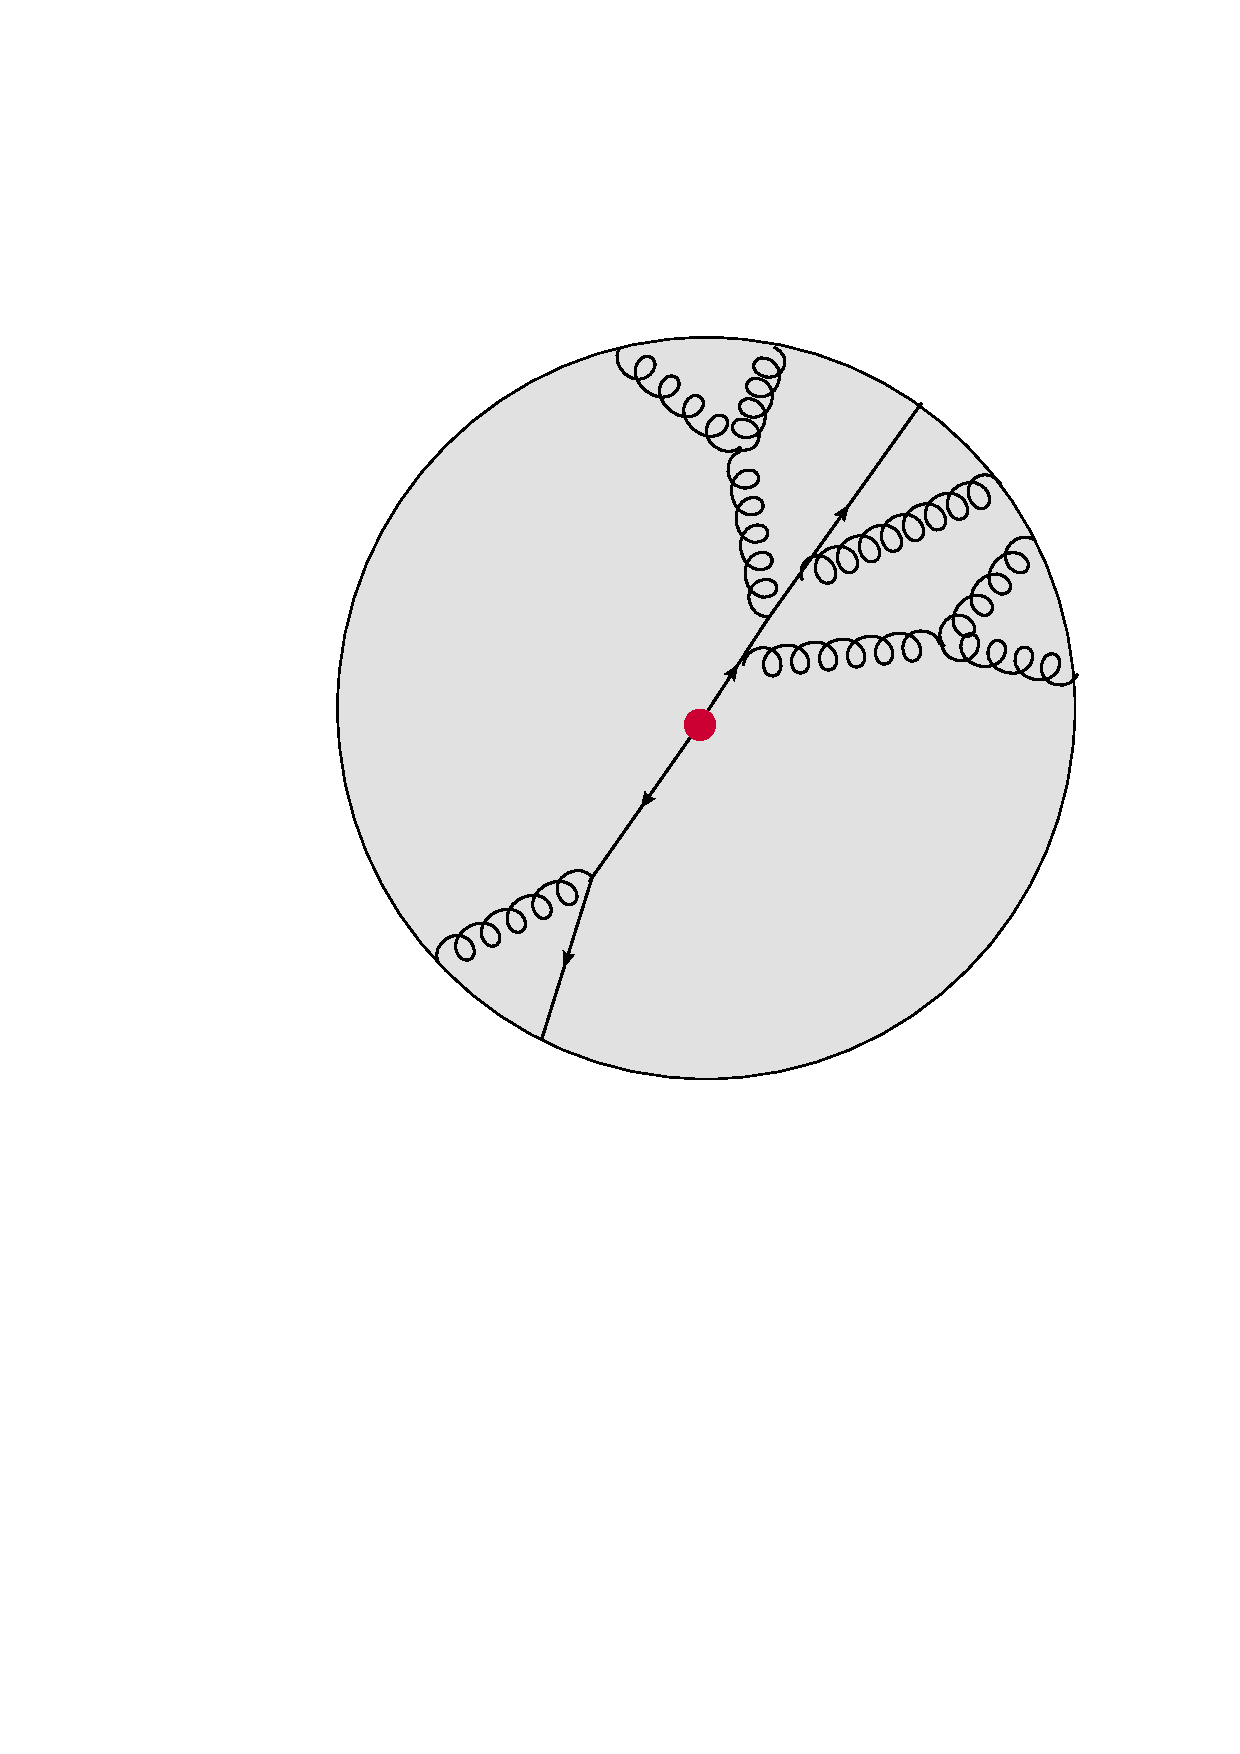
\includegraphics[width=.5\textwidth]{./PDF/Dijet_flucts2.pdf}}
\end{figure}
\end{column}

\end{columns}

\vspace*{-.2cm}

\item A recent Monte-Carlo study \textcolor{forestgreen}{\it\small (Milhano and Zapp,
arXiv:1512.08107)} 

\vspace*{.1cm}
 \begin{itemize}
\item \textcolor{violet}{fluctuations compete with path-length difference}

\end{itemize}
\vspace*{.1cm}
\item Analytic studies \textcolor{forestgreen}{\it\small (M. Escobedo and E.I., 
arXiv:1601.03629 \& 1609.06104)}

\vspace*{.1cm}
 \begin{itemize}
\item \textcolor{violet}{fluctuations in the energy loss are as large as the average value}

\end{itemize}


\end{itemize}
}

\subsection{}
\frame[t]{ \frametitle{\textbf{Medium-induced radiation}}
\vspace*{-.1cm}

\small
\begin{itemize}
\item Additional radiation triggered by interactions in the medium: \textcolor{red}{BDMPSZ}
 
 \vspace*{.05cm}
 %\hspace*{.8cm}
 \textcolor{forestgreen}{\it\small Baier, Dokshitzer, Mueller, Peign\'e, and
    Schiff;  Zakharov (96--97)}


\vspace*{.1cm}

\item Gluon emission is linked to \textcolor{red}{transverse
     momentum broadening}

\vspace*{.1cm}

\item Independent multiple scattering $\Longrightarrow$ \textcolor{red}{a random walk in $k_\perp$}


%\vspace*{.1cm}
 
%\vspace*{.2cm}
%\item  Uncertainty principle $\Longrightarrow$ \textcolor{red}{gluon formation time $t_{\rm f}$} 
  
  \vspace*{.05cm}
\begin{columns}[c]

\begin{column}{8.cm}

\vspace*{.1cm}

\begin{figure}%[h]
\centerline{%\hspace*{1.5cm}
\includegraphics[width=.8\textwidth]{./PDF/DemBranch2.pdf}}
\end{figure}
%\vspace*{-.7cm}

%
\end{column}

\begin{column}{5.cm}

 \vspace*{-.2cm}
 $$\hspace*{-1.cm}\textcolor{blue}{\langle k^2_\perp\rangle\simeq\,\hat q \,\Delta t}$$

 


%\vspace*{-.15cm}
%\vspace*{-.4cm}

 $$\hspace*{-1.cm}\textcolor{blue}{t_{\rm f}\,\simeq \,\frac{1}{\Delta E}
 \,\simeq \,\frac{\omega}{k_\perp^2}
  }$$
 
 \vspace*{.1cm}

 

\end{column}

\end{columns}

\vspace*{-.2cm}

\item The scatterings destroy quantum coherence and \textcolor{red}{favor gluon emissions}

 \vspace*{-.2cm}
  $$\hspace*{-.5cm}  \textcolor{blue}{t_{\rm f}\,\simeq\,\frac{\omega}{k_{\perp}^2}\quad \&
  \quad k_\perp^2\, \simeq\,\hat q t_{\rm f}\quad \Longrightarrow \quad} 
  \textcolor{red}{ t_{\rm f}(\omega)\,\simeq\,
   \sqrt{\frac{\omega}{\hat q}}}$$
   
   %\vspace*{-.1cm}

%\vspace*{.05cm}
%\item  \textcolor{violet}{softer gluons are emitted faster: \textcolor{blue}{LPM effect}}

% $$\hspace*{-1.cm}\textcolor{blue}{\hat q\simeq\,
 %\frac{m_D^2}{\lambda} \, \sim \, \alpha_s^2 T^3 \ln\frac{1}{\alpha_s}}$$
 
 
 %\vspace*{-.3cm}
 %$$\textcolor{blue}{ \hat q \simeq\,
 %\frac{m_D^2}{\lambda} \,=\,\frac{({\mbox{Debye mass}})^2}{{\mbox{
 %mean free path}}}\qquad\mbox{`jet quenching parameter'}}$$
 
 \normalsize

\end{itemize}
}

\subsection{}\frame[t]{ \frametitle{\textbf{Multiple branchings}}  %\vspace*{-.3cm}

\vspace*{-.15cm} 

\small
\begin{itemize}
%\item For sufficiently soft gluons, \textcolor{red}{multiple branching} becomes important

%\vspace*{.15cm}


\item Probability for emitting a gluon with \textcolor{red}{energy $\ge \omega$}
 during a \textcolor{red}{time $L$}

\vspace*{-.1cm}

$$%\hspace*{-1.3cm}
\textcolor{blue}{\mcal{P}(\omega, L) \simeq \as \,\frac{L}{t_{\rm f}(\omega)}
 \,\simeq\,\as\, L\,\sqrt{\frac{\hat q}{\omega}}
 }$$

%\vspace*{.15cm}
%\only<1>
 %\vspace*{.2cm}
%\vspace*{.1cm}
\item When \textcolor{red}{$\mcal{P}(\omega, L)\sim 1$}, multiple branching becomes important

\vspace*{-.1cm}

$$\textcolor{blue}{\omega \, \lesssim\, \omega_{\rm br}\equiv \alpha_s^2\hat q L^2\quad
\mbox{: the fundamental scale for what follows}
%\Longleftrightarrow\quad L\,\gtrsim\,\tbr(\omega)\equiv \frac{1}{\alpha_s}
%\sqrt{\frac{\omega}{\hat q}}
}$$

\vspace*{.1cm}

 \item LHC: the leading particle has  \textcolor{red}{$E\sim 100\,{\rm GeV}\,\gg\, \omega_{\rm br}
 \sim 5\div 10\,{\rm GeV}$} 
 
 
%\vspace*{.12cm}


\vspace*{.1cm}
\only<1>{\begin{figure}%[h]
\centerline{\hspace*{.5cm}
\includegraphics[width=.7\textwidth]{./PDF/Primaries_hard.pdf}}
\end{figure}
}

\only<2,3>{\begin{figure}%[h]
\centerline{\hspace*{.5cm}
\includegraphics[width=.7\textwidth]{./PDF/Primaries.pdf}}
\end{figure}
}


\vspace*{-.8cm}




\only<1>{\item In a \textcolor{red}{typical event}, the LP emits ... \begin{itemize}

\vspace*{.1cm}
\item 
\textcolor{violet}{a number of $\order{1}$ of gluons with \textcolor{red}{$\omega\sim \omega_{\rm br}$}}
\end{itemize}}

%\vspace*{.1cm}
\only<2>{\item In a \textcolor{red}{typical event}, the LP emits ... 
\begin{itemize}

\vspace*{.1cm}
\item 
\textcolor{violet}{a large number of softer gluons with \textcolor{red}{$\omega\ll \omega_{\rm br}$}}
\end{itemize}}


  
\only<3>{\item 
The energy loss is controlled by the 
  \textcolor{red}{hardest}  primary emissions}
  

\end{itemize}
}



\subsection{}\frame[t]{ \frametitle{\textbf{Democratic  branchings}}  %\vspace*{-.3cm}
\vspace*{-.3cm}

\textcolor{forestgreen}{\it\small J.-P.~Blaizot, E. I., Y.~Mehtar-Tani,
 PRL 111, 052001 (2013)}
 \vspace*{.1cm}
 
 \begin{itemize}
\item The primary gluons generate `mini-jets'
 via  \textcolor{red}{democratic branchings}

\vspace*{.1cm}
\begin{itemize}
\item \textcolor{violet}{daughter gluons carry comparable energy fractions:  \textcolor{red}{$z\sim 1-z\sim 1/2$}}

\vspace*{.15cm}
\item 
\textcolor{violet}{contrast to asymmetric splittings in the vacuum:  \textcolor{red}{$z\ll 1$}}

\end{itemize}

\vspace*{.05cm}

\begin{figure}%[h]
%\hspace*{-.6cm}
\centerline{
\includegraphics[width=.65\textwidth]{./PDF/CascadeEnergy3.pdf}}
\end{figure}

\vspace*{-.4cm}

\item Democratic branchings lead to \textcolor{red}{wave turbulence}

\vspace*{.1cm}
\begin{itemize}
\item \textcolor{violet}{energy flows from one parton generation to the next one,
at a rate which is independent of the generation}

\end{itemize}



\end{itemize}
}

\subsection{}\frame[t]{ \frametitle{\textbf{Energy loss at large angles}}  %\vspace*{-.3cm}
\vspace*{-.1cm}
 
 \begin{itemize}
\item Via successive democratic branchings, the 
energy is efficiently transmitted to softer and softer gluons,  \textcolor{red}{down 
to $\omega\sim T$} 

\vspace*{.1cm}
\begin{itemize}
\item \textcolor{violet}{the soft gluons  \textcolor{red}{thermalize}}   \
\textcolor{forestgreen}{\it\small (E.I. and Bin Wu, arXiv:1506.07871)}

\end{itemize}


\vspace*{.1cm}
\item 
\textcolor{blue}{Energy appears in many soft quanta propagating at large angles}
\vspace*{.1cm}

\begin{figure}%[h]
%\hspace*{-.6cm}
\centerline{
\includegraphics[width=.65\textwidth]{./PDF/CascadeEnergy3.pdf}}
\end{figure}

\vspace*{-.4cm}




%\vspace*{.1cm}
\item Medium-induced jet evolution $\approx$ \textcolor{blue}{a Markovien stochastic process}


   \vspace*{.15cm}
   \item What is the \textcolor{red}{average} energy loss and its \textcolor{red}{fluctuations} ?

\end{itemize}
}



\subsection{}\frame[t]{ \frametitle{\textbf{The average energy loss} }
\vspace*{-.1cm}

\small
\begin{itemize} 
\item Recall: energy loss is controlled by the primary emissions with
  \textcolor{red}{$\omega\sim \omega_{\rm br}$}
  
\vspace*{.1cm}
\begin{figure}%[h]
\centerline{\hspace*{.5cm}
\includegraphics[width=.7\textwidth]{./PDF/Primaries.pdf}}
\end{figure}


 \begin{itemize}

\vspace*{-.6cm}


\item \textcolor{violet}{softer emissions \textcolor{red}{($\omega\ll \omega_{\rm br}$)} carry very little
energy}


\vspace*{.15cm}


\item \textcolor{violet}{harder gluons \textcolor{red}{($\omega\gg \omega_{\rm br}$)} do not suffer
democratic branchings}

\vspace*{.05cm}\textcolor{violet}{$\Longrightarrow$ their energy remains at small angles}
\textcolor{red}{$\longrightarrow \Delta E_{_{\rm LPM}}$}


\end{itemize}


\vspace*{.05cm}

\item Confirmed by an exact calculation \textcolor{forestgreen}{\it\small (Blaizot, E. I., Mehtar-Tani,
 2013)}

 $$\textcolor{blue}{\langle \Delta E \rangle \,=\,
  E\left[1-\rme^{-\pi\frac{\omega_{\rm br}}{E}}\right]
    \,\simeq\,\pi \omega_{\rm br}} \uncover<2>{\textcolor{red}{\,=\,\pi \alpha^2_s \hat q L^2}}    
    $$
 
\uncover<2>{\begin{itemize}

\vspace*{-.3cm}
\item  \textcolor{violet}{independent of the \textcolor{red}{energy $E$} of the leading particle}
\vspace*{.15cm}
\item  \textcolor{violet}{rapidly increasing with the medium size \textcolor{red}{$\propto L^2$}}

%\vspace*{.15cm}
%\item  \textcolor{violet}{on the average, there are $\pi$ primary gluons with 
  %\textcolor{red}{$\omega\sim \omega_{\rm br}$}}
\end{itemize}
}
\end{itemize}
\normalsize
}

\subsection{}\frame[t]{ \frametitle{\textbf{Fluctuations in the energy loss at large angles} }
\vspace*{-.1cm}

\small
\begin{itemize} 
\item Recall: the probability for a primary emissions with $\omega\sim \omega_{\rm br}$ is of 
  \textcolor{red}{\textcolor{red}{$\order{1}$}}
  
\vspace*{.1cm}
\begin{figure}%[h]
\centerline{\hspace*{.5cm}
\includegraphics[width=.7\textwidth]{./PDF/Primaries.pdf}}
\end{figure}


 \begin{itemize}

\vspace*{-.6cm}


\item \textcolor{violet}{the  \textcolor{red}{average} number of such emissions
 is of \textcolor{red}{$\order{1}$} (indeed, it is $\pi$)}


\vspace*{.15cm}


\item \textcolor{violet}{successive such emissions are \textcolor{red}{quasi-independent}
($E \gg \omega_{\rm br}$)}
\end{itemize}


\vspace*{.05cm}
\item  \textcolor{red}{Fluctuations} in the number of such emissions
 must be of \textcolor{red}{$\order{1}$} as well 

\vspace*{.15cm}
\item Confirmed by exact calculations \textcolor{forestgreen}{\it\small (M. Escobedo and E. I., arXiv:1601.03629)}
 

 $$\textcolor{blue}{
 \sigma^2\,\equiv\,\langle{\Delta E}^2\rangle - 
 \langle \Delta E\rangle^2
 \,\simeq\,\frac{\pi^2}{3}\,\omega_{\rm br}^2\,=\,
 \textcolor{red}{\frac{1}{3} \langle \Delta E\rangle^2}}$$

    \vspace*{.1cm}
\item Variance is comparable to expectation value:
\textcolor{red}{large fluctuations} 

\end{itemize}
\normalsize
}

\subsection{}\frame[t]{ \frametitle{\textbf{Di-jet asymmetry from fluctuations}}  %\vspace*{-.3cm}
\vspace*{-.2cm}
 
 \begin{figure}%[h]
\centerline{\hspace*{.5cm}
\includegraphics[width=.7\textwidth]{./PDF/Dijet_flucts.pdf}}
\end{figure}
\vspace*{-.2cm}


 \small \begin{itemize}


\item  \textcolor{red}{Average} asymmetry is controlled by the \textcolor{red}{difference in path lengths} 
\vspace*{-.1cm}

$$\textcolor{blue}{\langle E_{1}-E_{2} \rangle \,=\,
\langle \Delta E_2-\Delta E_1 \rangle
\textcolor{red}{\,\propto\,\langle L_2^2-L_1^2\rangle}}$$

\vspace*{.1cm}

\item In experiments though, one rather measures \textcolor{red}{$|E_1-E_2|$}

%\vspace*{-.3cm}


$$\hspace*{-.5cm}
 \textcolor{blue}{\langle (E_{1}-E_{2})^2 \rangle -\langle E_{1}-E_{2} \rangle^2 
= \sigma^2_1+\sigma^2_2\,
%\propto \langle \Delta E_1\rangle^2+ \langle \Delta E_2\rangle^2
\textcolor{red}{\,\propto\,\langle L_2^2+L_1^2\rangle}
}$$

\vspace*{.1cm}

\only<1>{\item Fluctuations dominate whenever $L_1 \sim L_2$ (the \textcolor{red}{typical}
situation)}

%\vspace*{.15cm}
\only<2>{\item Difficult to check: no direct experimental control of $L_1$ and $L_2$}
\end{itemize}
\normalsize

}	 

\subsection{}\frame[t]{ \frametitle{\textbf{Monte-Carlo generated events (central collisions)}}  %\vspace*{-.3cm}
\vspace*{-.2cm}
 \textcolor{forestgreen}{\it\small (Milhano and Zapp, JEWEL,
arXiv:1512.08107)} \qquad  $\textcolor{blue}{A_{\rm J}=\frac{|E_{1}-E_{2}|}
{E_{1}+E_{2}}}$


 \begin{figure}%[h]
\centerline{%\hspace*{.5cm}
\includegraphics[width=.45\textwidth]{./PDF/MZ_Aj_killer.pdf}\quad
\includegraphics[width=.58\textwidth]{./PDF/MZ_DeltaLn.pdf}}
\end{figure}
\vspace*{-1.cm}

 \small \begin{itemize}


\item  \textcolor{violet}{Left:} Central production  \textcolor{red}{($L_1 = L_2$)} vs. randomly
distributed  production points  \textcolor{red}{(``full geometry'')}

\vspace*{.1cm}

\item  \textcolor{violet}{Right:} Distribution of  \textcolor{red}{$\Delta L\equiv L_1-L_2$} 
for di-jet events with different values for the asymmetry $A_J$

%\vspace*{.1cm}
\begin{itemize}

\item  \textcolor{violet}{the width of the distribution is a measure of fluctuations}
\end{itemize}

\end{itemize}
\normalsize
}


\subsection{}\frame[t]{ \frametitle{\textbf{Gluon multiplicities}}  %\vspace*{-.3cm}
%\vspace*{-.1cm}
 
  \begin{itemize}
% \small
 \item Average number of gluons with \textcolor{red}{$\omega\ge \omega_0$}
 
 \vspace*{.15cm}
\begin{itemize}
  \item \textcolor{violet}{ $\omega_0\ll E$ is the `resolution scale'}


%\vspace*{-.1cm}

 $$\textcolor{blue}{ \langle N(\omega_0)\rangle\,=\int_{\omega_0}^E\rmd \omega
\,\frac{\rmd N}{\rmd \omega}\,\simeq\,% 1+ \int_{x_0}^1\rmd x\,\frac{\tau}{x^{3/2}}\,=\,
1+2\left[\frac{\omega_{\rm br}}{\omega_0}\right]^{1/2}}
 \ \ \mbox{\textcolor{red}{(LP + radiation)}}$$
 
 \vspace*{.2cm}
  \item \textcolor{violet}{would be divergent if $\omega_0\to 0$}
\vspace*{.2cm}

 \item \textcolor{violet}{in experiments too, one has a non-zero resolution scale}
\vspace*{.2cm}

 \item \textcolor{violet}{independent of the energy $E$ of the LP}
\vspace*{.2cm}

\item \textcolor{violet}{$\langle N(\omega_0)\rangle\simeq 1$ when
$\omega_0\gg \omega_{\rm br}$ :} \textcolor{red}{just the leading particle}
\vspace*{.2cm}

\item \textcolor{violet}{$\langle N(\omega_0)\rangle\gg 1$ when
$\omega_0\ll \omega_{\rm br}$ :} \textcolor{red}{multiple branching}

\vspace*{.2cm}

\item \textcolor{violet}{amusingly enough: $\langle N(\omega_{\rm br})\rangle = 3 \simeq \pi$}
 \end{itemize}


 
 \vspace*{.15cm}
 \item Multiplicities are high for soft gluons: \textcolor{red}{$\omega_0\ll \omega_{\rm br}$}
  \end{itemize}
  
}


\subsection{}\frame[t]{ \frametitle{\textbf{Koba-Nielsen-Olesen scaling}}  %\vspace*{-.3cm}
\vspace*{-.2cm}
 
  \begin{itemize}
 \small

\item  One has similarly computed all the higher moments $\langle {N}^p\rangle$ with $p\ge 2$

 \vspace*{.1cm}
 \textcolor{forestgreen}{\it\small (M. Escobedo and E. I., arXiv:1609.06104)}

 \vspace*{.2cm}

\item For soft gluons, $\omega_0\ll \omega_{\rm br}$, they are all determined by the
1-point function:


\vspace*{.05cm}
$$\hspace*{-.5cm}\textcolor{blue}{\frac{\langle N^2\rangle}{\langle N \rangle^2}
\,\simeq\,\frac{3}{2}\,,\qquad
\frac{\langle {N}^p\rangle}{\langle{N}\rangle^p}
\,\simeq\,\frac{(p+1)!}{2^p}
}$$

\vspace*{.1cm}
\item \textcolor{red}{KNO scaling :} the reduced moments are pure numbers

\begin{itemize}
\vspace*{.1cm}
 \item  \textcolor{violet}{independent of any of the physical parameters of the problem}
   \end{itemize}

\vspace*{.1cm}
\item A special \textcolor{red}{negative binomial distribution} (parameter $r=2$)

\begin{itemize}
\vspace*{.1cm}
%\item \textcolor{violet}{jet in the vacuum : $r=3$ $\Longrightarrow$ the medium broadens the distribution}
 
% \vspace*{.15cm}
 \item  \textcolor{violet}{huge fluctuations (say, as compared to a Poissonian distribution)}

\vspace*{-.1cm}
$$\textcolor{blue}{\frac{\sigma_N}{\langle N\rangle}\Big |_{\rm KNO} \,=\,\frac{1}{\sqrt{2}}
\qquad {\rm vs.}\qquad \frac{\sigma_N}{\langle N\rangle}
\Big |_{\rm Poisson}\,=\,\frac{1}{\sqrt{\langle N\rangle}}}$$

%$$\textcolor{blue}{\sigma_N^2\equiv \langle N^2\rangle - \langle N \rangle^2\,\simeq\,
%\frac{1}{2}\langle N \rangle^2\qquad {\rm vs.}\quad \sigma_N^2=\langle N \rangle}$$
%\normalsize

 \end{itemize}
 
 \vspace*{.1cm}
\item KNO scaling also holds for a jet \textcolor{red}{in the vacuum} ...

\vspace*{.15cm}
\item ... but the medium-induced distribution is \textcolor{red}{much wider} !
  \end{itemize}
  
}


\subsection{}
\frame{ \frametitle{\textbf{Conclusions}} \vspace*{-.1cm}

\begin{itemize}
\vspace*{.1cm}

\item Effective theory and \textcolor{red}{physical picture} for jet quenching from \textcolor{red}{pQCD}

\begin{itemize}
\vspace*{.1cm}

\item \textcolor{violet}{event-by-event physics: multiple branching}
\vspace*{.15cm}

\item \textcolor{violet}{democratic branchings leading to wave turbulence}



\vspace*{.15cm}

\item \textcolor{violet}{thermalization of the soft branching products with $p\sim T$}

\vspace*{.15cm}

\item \textcolor{violet}{efficient transmission of energy to large angles}

\vspace*{.15cm}

\item \textcolor{violet}{wide probability distribution, strong fluctuations, KNO scaling}

%\vspace*{.15cm}
\end{itemize}

\vspace*{.15cm}

\item \textcolor{red}{Fluctuations} compete with the \textcolor{red}{difference in path lengths}
in determining the di-jet asymmetry 

\vspace*{.2cm}
\item Qualitative and semi-quantitative agreement with the phenomenology of 
\textcolor{red}{di-jet asymmetry at the LHC}

\vspace*{.2cm} 
\item Important dynamical information still missing:  \textcolor{red}{vacuum-like
radiation (parton virtualities), medium expansion ...} 
\end{itemize}
}





\end{document}
\subsection{}\frame[t]{ \frametitle{\textbf{Probabilistic picture}}  \vspace*{-.15cm}
	
	 \begin{itemize}

\item Medium-induced jet evolution $\approx$ \textcolor{red}{a Markovien stochastic process}

\vspace*{.1cm}

 \begin{itemize}
 
 \item \textcolor{violet}{a sequence of independent branchings occurring with BDMPSZ rate}

%\vspace*{.15cm}

\end{itemize}

\vspace*{.1cm}
\item It can be studied via \textcolor{red}{Monte-Carlo} 
\textcolor{forestgreen}{\small\it (Schenke, Gale, Jeon, `MARTINI', '09)}

\vspace*{.1cm}

 \begin{itemize}
 
 \item \textcolor{violet}{but such numerical studies missed interesting but subtle phenomena}

%\vspace*{.15cm}

\end{itemize}

\vspace*{.1cm}
\item Infinite hierarchy of equations for \textcolor{red}{$n$-point correlation functions}

\small
$$\hspace*{-.5cm}
\textcolor{blue}{
D(x,t)\equiv x\,\left\langle \frac{\rmd N}{\rmd x}(t)\right\rangle\,,
\qquad
D^{(2)}(x,x',t)\equiv x x'\,\left\langle \frac{\rmd N_{\rm pair}}{\rmd x \,\rmd x'}(t)\right\rangle
}$$
\normalsize


%\vspace*{.1cm}

\begin{itemize}
 
 \item \textcolor{violet}{easy to write ... and possible to solve  \textcolor{red}{analytically}}


%\vspace*{.15cm}
\vspace*{.1cm}
\textcolor{forestgreen}{\it\small J.-P.~Blaizot, E. I., Y.~Mehtar-Tani,
 PRL 111, 052001 (2013)}
 
 \vspace*{.1cm}

\textcolor{forestgreen}{\it\small M. Escobedo and E. I., arXiv:1601.03629  \& work in progress}

 
\end{itemize}
\vspace*{.1cm}
\item These solutions revealed interesting \textcolor{red}{new phenomena}

\begin{itemize}
 
 \item \textcolor{violet}{wave turbulence, KNO scaling, large fluctuations ...}
\end{itemize}

\end{itemize}
	}


\subsection{}\frame[t]{ \frametitle{\textbf{The gluon spectrum $D(x)$}}  \vspace*{-.1cm}
	
\small	 \begin{itemize}

\item Kinetic equation for  $D(x,t)$ \textcolor{violet}{($x=\omega/E$ : energy fraction of a gluon)}

\vspace*{-.1cm}
$$\textcolor{blue}{\frac{\partial}{\partial t} D(x,t)
\, = \,\frac{1}{t_{\rm br}(x)}\int_0^1\frac{\rmd z} {\sqrt{z}(1-z)^{\frac{3}{2}}} 
 %\,  {\cal K}(x)
 \left[
D\left(\frac{x}{z},t\right) - \sqrt{z} D(x,t) \right]}$$

\vspace*{.1cm}
\item Linear equation: `gain' - `loss'
\vspace*{.1cm}
\begin{figure}%[h]
\centerline{
\includegraphics[width=.9\textwidth]{./PDF/Branching_GainLoss}}
\end{figure}


\vspace*{-.6cm}
\item Branching rate = the inverse of the democratic branching time $\tbr(x)$

\vspace*{.15cm}
\item Initial condition: \textcolor{blue}{${D(x,t=0)=\delta(x-1)}$}

\vspace*{.15cm}
\item \textcolor{red}{Turbulent fixed point:} the r.h.s. vanishes for
\textcolor{red}{$D(x) = \frac{1}{\sqrt{x}}$}



\vspace*{.15cm}
\item Exact solution:
\textcolor{forestgreen}{\it\small J.-P.~Blaizot, E. I., Y.~Mehtar-Tani,
 2013}
\end{itemize}
\normalsize
	}
	
	
	\subsection{}\frame[t]{ \frametitle{\textbf{Gluon spectrum}}  \vspace*{-.4cm}




 
$$\textcolor{blue}{D(x,\tau)\,=\,\frac{\tau}{\sqrt{x}(1-x)^{3/2}}\ \rme^{-\pi\frac{\tau^2}{1-x}}\,,\qquad
\textcolor{violet}{x\equiv\frac{p}{E}\,,\ \
\tau\equiv \frac{t}{t_{\rm br}(E)}}}$$
\vspace*{.02cm}

\begin{itemize}
\item Leading particle peak near \textcolor{red}{$x=1$} at early times  \textcolor{red}{$\tau \ll 1$}
\vspace*{.2cm}
\item Power-law spectrum $\textcolor{red}{D\propto {1}/{\sqrt{x}}}$ at \textcolor{red}{$x\ll 1$}
%\vspace*{.2cm}
%\end{itemize}

%\vspace*{-.2cm}
\begin{figure}%[h]
\centerline{
\includegraphics[width=.6\textwidth]{./PDF/D0_t1}}
\end{figure}

\vspace*{-1.1cm}
\centerline{\small $\tau = 0.1$}
\end{itemize}
}

\subsection{}\frame[t]{ \frametitle{\textbf{Early times  $t \lesssim \tbr(E)$}}  
\vspace*{-.2cm}




 
$$\textcolor{blue}{D(x,\tau)\,=\,\frac{\tau}{\sqrt{x}(1-x)^{3/2}}\ \rme^{-\pi\frac{\tau^2}{1-x}}\,,\qquad
\textcolor{violet}{x\equiv\frac{p}{E}\,,\ \
\tau\equiv \frac{t}{t_{\rm br}(E)}}}$$
%\vspace*{.05cm}

\begin{itemize}
\vspace*{.2cm}


\item Increasing $t$: the LP peaks decreases, broadens, and moves to the left

\vspace*{.2cm}
\only<1>{\item The shape at small $x$ is not changing:  \textcolor{red}{genuine fixed point}}

\only<2>{\item When  \textcolor{red}{$t\sim \tbr(E)$}, the LP disappears via democratic branching}

\vspace*{-.1cm}

\only<1>{\begin{figure}%[h]
\centerline{
\includegraphics[width=.6\textwidth]{./PDF/D0_t3}}
\end{figure}

\vspace*{-1.1cm}
\centerline{\small $\tau = 0.1$,\, \textcolor{violet}{0.2}, \,\textcolor{blue}{0.4} }
}

\only<2>{\begin{figure}%[h]
\centerline{
\includegraphics[width=.6\textwidth]{./PDF/D0_t4}}
\end{figure}
\vspace*{-1.1cm}
\centerline{\small $\tau = 0.1$,\, \textcolor{violet}{0.2}, \,\textcolor{blue}{0.4}, \,\textcolor{red}{0.8} }
}

\end{itemize}
}


\subsection{}\frame[t]{ \frametitle{\textbf{Later times $t > \tbr(E)$}}  
\vspace*{-.4cm}




 
$$\textcolor{blue}{D(x,\tau)\,\simeq\,\frac{\tau}{\sqrt{x}}\ \rme^{-\pi{\tau^2}}\,,\qquad
\textcolor{violet}{x\equiv\frac{p}{E}\,,\ \
\tau\equiv \frac{t}{t_{\rm br}(E)}}}$$
%\vspace*{.05cm}

\begin{itemize}
%\vspace*{.2cm}

\only<1>{\item The spectrum shrinks towards small \textcolor{red}{$x\lesssim 1/\tau$}

\vspace*{.2cm}

\item  Its strength is uniformly suppressed with increasing $\tau$}
 
%\vspace*{.2cm}

\only<2->{\item The energy flows out of the spectrum
\vspace*{.2cm}

\item \textcolor{red}{ Where does the energy go ?}

%\item It accumulates into a condensate at $x=0$:  \textcolor{red}{`perfect sink'}
}

\vspace*{-.2cm}


\only<1>{\begin{figure}%[h]
\centerline{
\includegraphics[width=.6\textwidth]{./PDF/D0_t5}}
\end{figure}
\vspace*{-1.2cm}
\centerline{\small $\tau = 0.1$,\, \textcolor{violet}{0.2}, \,\textcolor{blue}{0.4}, \,\textcolor{red}{0.8},
\,\textcolor{brown}{1} }
}

\only<2>{\begin{figure}%[h]
\centerline{
\includegraphics[width=.6\textwidth]{./PDF/D0_t6}}
\end{figure}
\vspace*{-1.2cm}
\centerline{\small $\tau = 0.1$,\, \textcolor{violet}{0.2}, \,\textcolor{blue}{0.4}, \,\textcolor{red}{0.8},
\,\textcolor{brown}{1},
\,\textcolor{forestgreen}{1.2} }
}

%
%\textcolor{violet}{$\hspace*{-.5cm}\int_0^1\rmd x\,D(x,t)=1\ \,\mbox{for any $t$}$}


\vspace*{-.9cm}

\end{itemize}
}



\subsection{}\frame[t]{ \frametitle{\textbf{Wave turbulence}}
\vspace*{-.15cm}

\begin{itemize}
	\item Fixed point \textcolor{red}{$D(x) = \frac{1}{\sqrt{x}}$} $\Rightarrow$
	%`gain = `loss'  $\Rightarrow$
	Energy flux is independent of $x$ %: \textcolor{red}{wave turbulence}

 \begin{itemize}

\vspace*{.1cm}


\item \textcolor{violet}{energy flows from one parton generation to the next one, without accumulating
at any intermediate value of $x$}


\vspace*{.15cm}


\item \textcolor{violet}{formally it accumulates into a condensate at $x=0$}

\vspace*{.15cm}


\item \textcolor{violet}{physically, it thermalizes}
\end{itemize}

\vspace*{.2cm}

\begin{columns}[c]

\begin{column}{6.5cm}

%\vspace*{.2cm}
\begin{figure}%[h]
\centerline{%\hspace*{1.5cm}
\includegraphics[width=.65\textwidth]{./PDF/Branching_democratic_1.pdf}}
\end{figure}
\vspace*{-.7cm}

%
\end{column}

\begin{column}{7.cm}


\vspace*{-.3cm}
\begin{figure}%[h]
\centerline{\hspace*{-.6cm}
\includegraphics[width=.7\textwidth]{Richardson_cascade.png}}
\end{figure}
\vspace*{-1.cm}

%\centerline{\textcolor{violet}{breaking-up vortices}}
%\vspace*{-.3cm}

 
 \end{column}

\end{columns}
\vspace*{.3cm}
\item The prototype: Richardson cascade for breaking-up vortices




\end{itemize}
}



	\subsection{}\frame[t]{ \frametitle{\textbf{Correlations \& fluctuations}}  \vspace*{-.15cm}
	
	 \begin{itemize}
	 
	 \item  \textcolor{red}{Exactly, analytic, solutions} for all the $n$-point correlations
	% \begin{itemize}

\vspace*{.1cm}

\textcolor{forestgreen}{\it\small M. Escobedo and E. I., arXiv:1601.03629  \& work in progress}
%\vspace*{-.1cm}
%\end{itemize}

\vspace*{.15cm}


\only<1>{ \item The 2-point correlation \textcolor{red}{(the gluon pair density)}
 
% \vspace*{-.2cm}

\small
 $$\textcolor{blue}{D^{(2)}(x,x',\tau)\,=\,\frac{1}{2\pi}\frac{1}{\sqrt{x x' (1-x-x')}}\left[\rme^{-\frac{\pi\tau^2}{1-x-x'}}
   -\rme^{-\frac{4\pi\tau^2}{1-x-x'}}\right]}$$
\normalsize
}
  
 %\vspace*{.1cm}
 \item Physical interpretation: correlations due to \textcolor{red}{common ancestors}
 
  \vspace*{.15cm}

  % \vspace*{.05cm}
%\uncover<2>
{\begin{columns}[c]

\begin{column}{6.5cm}

%\vspace*{.1cm}
\vspace*{-.25cm}
\begin{figure}%[h]
\centerline{%\hspace*{1.5cm}
\includegraphics[width=.8\textwidth]{./PDF/JetCorrel1.pdf}}
\end{figure}
%\vspace*{-.7cm}

%
\end{column}

\begin{column}{6.5cm}


%\vspace*{-.15cm}
\begin{figure}%[h]
\centerline{\hspace*{-.5cm}
\includegraphics[width=.75\textwidth]{./PDF/JetCorrel3.pdf}}
\end{figure}
 


\end{column}

\end{columns}

\vspace*{-.2cm}

\begin{itemize}
\item \textcolor{violet}
{gluons from a same mini-jet are correlated with each other}

\vspace*{.15cm}
\item \textcolor{violet}{those from
different mini-jets are quasi-independent}
 \end{itemize}
 }
  \end{itemize}
}



	\subsection{}
\frame[t]{ \frametitle{\textbf{Di--jet asymmetry : $A_{\rm J}$}
\textcolor{green}{\it (CMS)}} \vspace*{-.3cm}

%\textcolor{red}{\Large Elliptic flow \& Jet quenching}
\begin{figure}%[h]
\centerline{
\includegraphics[width=.65\textwidth]{./JETS/CMS_dijet_AJ.pdf}}
\end{figure}
\vspace*{-.6cm}
\begin{itemize}

\item   Event fraction as a function of the di--jet energy imbalance
    in \textcolor{red}{p+p (a)} and \textcolor{red}{Pb+Pb (b--f)}
    collisions for different bins of centrality

  \vspace*{-.05cm}
$$\textcolor{blue}{A_{\rm J}=\frac{E_{1}-E_{2}}
{E_{1}+E_{2}}\qquad (E_i\equiv p_{T,i} =\ 
\mbox{jet energies})}$$

\vspace*{.15cm}
\only<1>{\item N.B. A pronounced asymmetry  already in  \textcolor{red}{p+p} (3-jet events)}
\only<2>{\item \textcolor{red}{Central Pb+Pb :} the asymmetric events occur more often}
\end{itemize} }



\subsection{}\frame[t]{ \frametitle{\textbf{Energy imbalance @ large angles: $R=0.8$}} 
\vspace*{-.3cm}
%\item The energy imbalance for a jet with a wide opening : \textcolor{red}{$R=0.8$}

%\vspace*{.1cm}
  \begin{figure}[tb]
\centerline{%\hspace*{0.4cm}
\includegraphics[width=1.1\textwidth]{./PDF/CMS_DiJet_LargeAngle.pdf}}
\end{figure}
\vspace*{-.5cm}

\begin{itemize}

\item No missing energy : \textcolor{red}{$E_{\rm Lead}^{\textcolor{blue}{\rm in+out}}
\, =\, E_{\rm SubLead}^{\textcolor{blue}{\rm in+out}}$ } 
%(hard particles)
\vspace*{.25cm}

\item In-Cone : \textcolor{red}{$E_{\rm Lead}^{\textcolor{blue}{\rm in}}\, > \, E_{\rm SubLead}^
{\textcolor{blue}{\rm in}}$ } : {di-jet asymmetry, hard particles}
\vspace*{.25cm}


\item Out-of-Cone : \textcolor{red}{$E_{\rm Lead}^{\textcolor{blue}{\rm out}}\, < \, E_{\rm SubLead}^
{\textcolor{blue}{\rm out}}$ } : {soft hadrons @ large angles}


\end{itemize}
}



\end{document}

\subsection{}\frame[t]{ \frametitle{\textbf{A challenge for the theorists}}  %\vspace*{-.3cm}
\vspace*{-.15cm}
 
 \begin{itemize}
\item Soft hadrons can be easily deviated towards large angles:

  \textcolor{red}{elastic scatterings
with the medium constituents}

 
\vspace*{.2cm} \item Main question: how is that possible that
a \textcolor{red}{significant} fraction of the jet
energy be carried by its \textcolor{red}{soft} constituents ?

\vspace*{.2cm}
\item Recall: \textcolor{red}{bremsstrahlung in the vacuum} 
\textcolor{forestgreen}{($\omega =xE$, $\theta\simeq \kk/\omega$)}
\vspace*{.1cm}


 \vspace*{.05cm}
\begin{columns}[c]

\begin{column}{8.cm}

\vspace*{.1cm}

\begin{figure}%[h]
\centerline{%\hspace*{1.5cm}
\includegraphics[width=.85\textwidth]{./PDF/JetVacuum.pdf}}
\end{figure}
%\vspace*{-.7cm}

%
\end{column}

\begin{column}{5.cm}


%\vspace*{-.15cm}
\vspace*{-.4cm}

$$\hspace*{-1.cm}
\textcolor{blue}{{\rmd \mcal{P}}\,=\,\frac{\alpha_s C_R}{\pi}\ \frac{\rmd x}{x}
\ \frac{\rmd\kk^2}{\kk^2}
}$$

 


\end{column}

\end{columns}

\only<1>{\vspace*{-.2cm}


\begin{itemize} \item \textcolor{violet}{many soft gluons ... which however carry very little energy}

\vspace*{.15cm}
\item  \textcolor{violet}{asymmetric splittings  $x\ll 1$ : energy remains in the parent partons}

\vspace*{.15cm}
\item \textcolor{violet}{angular ordering due to destructive interferences}

\end{itemize}}

\only<2>{\vspace*{-.05cm}

\item Jet in the vacuum are \textcolor{red}{well collimated}
\vspace*{.15cm}
\item How is this picture modified for  \textcolor{red}{jets in a medium} ?
}

\end{itemize}

}





\subsection{}\frame[t]{ \frametitle{\textbf{Adding elastic collisions}}  %\vspace*{-.3cm}
\vspace*{-.2cm}
 
 \begin{itemize}
 \item So far, collisions used only to trigger emissions \textcolor{red}{(`inelastic collisions')}
 
 \vspace*{.2cm}

\only<1>{\begin{figure}%[h]
\centerline{%\hspace*{1.5cm}
\includegraphics[width=.5\textwidth]{./PDF/InducedBranch.pdf}}
\end{figure}
}

\only<2>{

\begin{columns}[c]

\begin{column}{7.5cm}


\vspace*{.2cm}

\begin{figure}%[h]
\hspace*{-.2cm}
\centerline{
\includegraphics[width=.8\textwidth]{./PDF/LangevinG.pdf}}
\end{figure}


%\vspace*{-.5cm}




%\vspace*{-.2cm}

\end{column}


\begin{column}{6.5cm}

\vspace*{-.2cm}
 $$\hspace*{-1.cm}\textcolor{blue}{\langle p^2_\perp(t)\rangle\simeq\,\hat q \,t}$$


\vspace*{-.2cm}

 $$\hspace*{-1.cm}\textcolor{blue}{\langle p_z(t)\rangle\simeq p_0 -\eta t}$$
 
 \vspace*{-.2cm}
 $$\hspace*{-1.cm}\textcolor{blue}{\langle \Delta p^2_z(t)\rangle\simeq\,\hat q_\ell t}$$
 
  
 %\vspace*{-.1cm}
 
\end{column}
\end{columns}


\vspace*{.3cm}
\item Elastic collisions too can redistribute energy and momentum 

 \vspace*{.1cm}
\textcolor{red}{$\Longrightarrow$
 collisional energy loss and momentum broadening}

\vspace*{.15cm}
\item The jet particles are relatively hard to start with: \textcolor{red}{$\omega\simeq p_z\gg T$}
 \vspace*{.15cm}
 
	\item Small angle scattering (Langevin) :  \textcolor{red}{`drag' \& `diffusion'}

\vspace*{.2cm}

\item The medium is in thermal equilibrium $\Rightarrow$ \textcolor{red}{Einstein relation:}
$\textcolor{red}{\hat q_\ell=2T\eta}$

\vspace*{.2cm}

\item A test particle eventually \textcolor{blue}{thermalizes} : \textcolor{red}{$f_p\propto \rme^{-p/T}$}

}
\end{itemize}

}

\subsection{}\frame[t]{ \frametitle{\textbf{Thermalization of a test particle}}  %\vspace*{-.3cm}
\vspace*{-.1cm}
 
 \begin{itemize}
 \item An energetic test particle which is not allowed to radiate


%\vspace*{.2cm}
\begin{columns}[c]

\begin{column}{7.5cm}


\vspace*{.2cm}

\begin{figure}%[h]
\hspace*{-.2cm}
\centerline{
\includegraphics[width=.8\textwidth]{./PDF/LangevinG.pdf}}
\end{figure}


%\vspace*{-.5cm}




%\vspace*{-.2cm}

\end{column}


\begin{column}{6.5cm}

\vspace*{-.2cm}

 $$\hspace*{-1.cm}\textcolor{blue}{\langle p_z(t)\rangle\simeq p_0 -\eta t}$$
 
 \vspace*{-.2cm}
 $$\hspace*{-1.cm}\textcolor{blue}{\langle \Delta p^2_z(t)\rangle\simeq\,\hat q_\ell t}$$
 
 %\vspace*{-.2cm}
 %$$\hspace*{-1.cm}\textcolor{blue}{\langle p^2_\perp(t)\rangle\simeq\,\hat q \,t}$$

 
 %\vspace*{-.1cm}
 
\end{column}
\end{columns}

\vspace*{.25cm}
\item The test particle thermalizes via elastic collisions :

%
\vspace*{.1cm}
\begin{itemize}
 \item \textcolor{violet}{first, it loses most of its energy via drag, 
over a time \textcolor{red}{$\tth(p_0)$}}
 \vspace*{-.1cm}


 $$\textcolor{blue}{\tth(p_0)\,\simeq\,\frac{p_0}{\eta}\,=\,\frac{2p_0 T}{\hat q_\ell}\,
\uncover<2>{ \textcolor{red}{=\,\frac{p_0}{T}\,\trel\,\gg\,\trel}}
}$$
 
 \vspace*{.1cm}
 \item \textcolor{violet}{then, it approaches a thermal distribution, over an additional time \textcolor{red}{$\trel$}}
  \end{itemize}



 
 \vspace*{-.2cm}
  $$\textcolor{blue}{ \trel \equiv
 \frac{2T^2}{\hat q_\ell}\,\sim\,\frac{1}{ \alpha_s^2 T \ln(1/\alpha_s)}}$$
 
\uncover<2>{  \vspace*{.1cm} \item Overall duration controlled by the 1st stage:
 \textcolor{red}{collisional energy loss}}

\end{itemize}

%\end{itemize}
}

\subsection{}\frame[t]{ \frametitle{\textbf{Restoring the branchings}}  %\vspace*{-.3cm}
\vspace*{-.5cm}

\only<1>{\begin{columns}[c]

\begin{column}{7.5cm}


\vspace*{.2cm}

\begin{figure}%[h]
\hspace*{-.2cm}
\centerline{
\includegraphics[width=.8\textwidth]{./PDF/InducedBranch.pdf}}
\end{figure}


%\vspace*{-.5cm}




%\vspace*{-.2cm}

\end{column}


\begin{column}{6.5cm}

\vspace*{-.2cm}

 $$\hspace*{-1.cm}\textcolor{blue}{\tbr(p) \,\sim\, \sqrt{\frac{T}{p}}\,\tth(p)
}
 $$
 
% \vspace*{-.1cm}
 %$$\hspace*{-1.cm} \textcolor{red}{\tbr(p) \ll \tth(p) \ \mbox{if $p\gg T$}}$$
 
 %\vspace*{-.2cm}
 %$$\hspace*{-1.cm}\textcolor{blue}{\langle p^2_\perp(t)\rangle\simeq\,\hat q \,t}$$

 
 %\vspace*{-.1cm}
 
\end{column}
\end{columns}
\vspace*{.25cm}}

\only<2>{\vspace*{.4cm}
	\begin{figure}%[h]
%\hspace*{-.6cm}
\centerline{
\includegraphics[width=.8\textwidth]{./PDF/Coll_Inelastic_Gain.pdf}}
\end{figure}
\vspace*{-.2cm}
}



 
 \begin{itemize}
 \item Hard gluons \textcolor{red}{($p\gg T$)}
 branch before losing much energy via drag

 \begin{itemize}

\vspace*{0.1cm}
\item \textcolor{violet}{thermalization effects are irrelevant for the hard gluons}

\vspace*{.15cm}
\item \textcolor{violet}{democratic branching is more efficient than drag for degrading energy}

\end{itemize}
\vspace*{.1cm}
 \item When \textcolor{red}{$p\lesssim T$}, the 2 types of processes
 compete with each other:

\vspace*{-.2cm}
$$\textcolor{blue}{\tth(T)\,\sim \,\tbr(T)\,\sim\,\trel}$$ 
 
\vspace*{.1cm} \begin{itemize}


%\vspace*{.15cm}
\item \textcolor{violet}{soft gluons expected to thermalize within an interval $\sim\trel$}
   
   \vspace*{.15cm}
\item \textcolor{violet}{when/if this happens, the branching process stops at the scale $T$}

 \vspace*{.15cm}
\item \textcolor{violet}{compensation between splitting ($1\to 2$) and recombination ($2\to 1$)}
\end{itemize}

%\vspace*{.1cm}
 %\item The time scale for thermalizing a mini-jet is controlled by \textcolor{red}{branchings}
 
 
\end{itemize}
}


\subsection{}\frame[t]{ \frametitle{\textbf{Kinetic theory for jet evolution}}  \vspace*{-.2cm}
\begin{itemize}
\item The relevant dynamics can be encoded into a \textcolor{red}{kinetic equation}

\vspace*{.1cm}
\textcolor{forestgreen}{\small\it  Baier, Mueller, Schiff, Son '01 (`bottom-up');
Arnold, Moore, Yaffe, '03}

$$\textcolor{blue}{ \left(\frac{\partial}{\partial t}+{\bm v}\cdot \nabla_{\bm x} \right)f(t,\bx,\bp)\, =\, \mcal{C}_{\rm el}[f]+
\mcal{C}_{\rm br}[f]}$$

\item \textcolor{red}{$f(t,\bx,\bp)$ :} gluon occupation number (jet + medium)

\vspace*{.15cm}
\item Used in studies of the \textcolor{red}{QGP thermalization}
\textcolor{forestgreen}{\small\it Kurkela et al (2014-15)}

\vspace*{.15cm}
\item The jet problem is further complicated by its  \textcolor{red}{strong inhomogeneity}

$$\textcolor{blue}{ f(t=0,\bx,\bp)\,=\,%\frac{(2\pi)^3}{2(N_c^2-1)}\,
\delta^{(3)}(\bx)\,
\delta^{(2)}(\bp_\perp)\,\delta(p_z-E)}$$

\vspace*{.1cm}
%\item Understand the relevant \textcolor{red}{time scales} and write some simpler equations


\item A tractable and physically meaningful equation can be obtained by projecting the dynamics along the 
\textcolor{red}{longitudinal (jet) axis}

 
 \vspace*{.1cm}
  \textcolor{forestgreen}{\it\small (E.I. and Bin Wu, arXiv:1506.07871)}


\vspace*{.15cm}
\item Parametrically correct down
to \textcolor{red}{$p\sim T$} (captures the right time scales)
\end{itemize}
}


	\subsection{}\frame[t]{ \frametitle{\textbf{A longitudinal kinetic equation}}  %\vspace*{-.3cm}
\vspace*{-.1cm}
 
 \begin{itemize}
 \item Important simplifications occurring when \textcolor{red}{$p\gg T$} :  \begin{itemize}
\vspace*{.15cm}
\item \textcolor{violet}{the gluons from the jet can be distinguished from those in the medium}


 \vspace*{.15cm}

\item \textcolor{violet}{occupation numbers are small : $f(t,\bx,\bp)  \ll 1$
 $\Longrightarrow$ \textcolor{blue}{linear equation}}
 
 
 \vspace*{.15cm}
 \item \textcolor{violet}{\textcolor{blue}{$p_z \gg p_\perp$} $\Longrightarrow$
$p_z\simeq p$ controls the time scales for branchings}

 \vspace*{.15cm}
 \item \textcolor{violet}{one can restrict oneself to the \textcolor{blue}{longitudinal dynamics} :
  \textcolor{red}{$f(t,z,p_z)$}}

\end{itemize}

\vspace*{-.1cm}
\begin{align}\label{eq:equationL}
&\textcolor{red}{\left(\frac{\partial}{\partial t} +v_z\frac{\partial}{\partial z} \right)f(t,z,p_z)
\, = \frac{\hat{q}}{4}\,\frac{\partial}{\partial {p_z}}\left[\left(\frac{\partial}{\partial {p_z}} + \frac{v_z}{T}\right) f \right]}\nonumber\\*[0.3cm]
&\qquad\qquad\qquad
\textcolor{red}{+\frac{1}{t_{\rm br}(p_z)}\int_{p_*} \frac{\rmd x} {[x(1-x)]^{\frac{3}{2}}} 
 %\,  {\cal K}(x)
 \left[\frac{1}{\sqrt{x}}\,
f\left(\frac{p_z}{x}\right) - \frac{1}{2} f(p_z) \right]}\nonumber
\end{align}

\vspace*{.15cm}

\begin{itemize}
%\vspace*{-.1cm}

\item \textcolor{violet}{drift, elastic collisions \textcolor{violet}{(diffusion \& drag)},  branchings (gain \& loss)}

\vspace*{.15cm}

\item \textcolor{violet}{branching process cut off by hand at a scale \textcolor{blue}{$p_*\sim T$}}

\end{itemize}

\vspace*{.1cm}
\item Parametrically correct down
to \textcolor{red}{$p_z\sim T$} (captures the right time scales)

\vspace*{.1cm}


 % \end{itemize}


\end{itemize}
	}
	
	
	
	\subsection{}
\frame{ \frametitle{\textbf{The source approximation}} %\vspace*{-.15cm}

	
\begin{itemize}

\item The branching process $\approx$ a \textcolor{red}{source} of gluons with $p=p_*\gtrsim T$
\vspace*{.1cm}

\begin{itemize}
%\vspace*{.1cm}

\item \textcolor{violet}{gluons with $p\gg T$ are not significantly affected by collisions}

\vspace*{.2cm}

\item \textcolor{violet}{the branching process gets extinct around $p\sim T$  in the approach
to thermal equilibrium}
\end{itemize}

\vspace*{.15cm}\item The steady source approximation:  %\textcolor{red}{exact solution}

	$$\hspace*{-.5cm}\textcolor{blue}{\left(\frac{\partial}{\partial t}+v\frac{\partial}{\partial z} \right)f
 = \frac{\hat{q}}{4}\frac{\partial}{\partial {p}}\left[\left(\frac{\partial}{\partial {p}} + \frac{v}{T}\right) f \right]
+ } \textcolor{red}{\,T\delta(t-z)\delta(p- p_*)%\,\Gamma_0
}$$

\vspace*{.15cm}

\item 1-dimensional ultrarelativistic Fokker-Planck equation:  \textcolor{red}{exact solution}

\vspace*{.1cm}
 \begin{itemize}
%\vspace*{.1cm}

\item \textcolor{violet}{characteristic distribution: a `front' and a `tail'}

\vspace*{.1cm}

\item \textcolor{violet}{also recovered with dynamical branchings}
\end{itemize}

\end{itemize}
}

	
	\subsection{}
\frame{ \frametitle{\textbf{The front \& the tail}} \vspace*{-.15cm}

\vspace*{-.15cm}
\begin{figure}%[h]
\centerline{
\includegraphics[width=.7\textwidth]{./PDF/sourced.png}}
\end{figure}
\vspace*{-1.2cm}

\begin{itemize}

\vspace*{.1cm}\item \textcolor{red}{The front $\,\propto \delta(t-z)$ :}  gluons with $T\lesssim p < p_*$


\vspace*{.1cm}
 \begin{itemize}
%\vspace*{.1cm}

\item \textcolor{violet}{gluons recently injected that had no time to thermalize}
\end{itemize}


\vspace*{.15cm} \item \textcolor{red}{A tail at $z \lesssim t-\trel$ :} $f_p\propto \rme^{-|p|/T}$

\vspace*{.1cm}
\begin{itemize}
%\vspace*{.1cm}

\item \textcolor{violet}{gluons in thermal equilibrium with the medium}
\end{itemize}
\end{itemize}

}

	
	
\subsection{}\frame[t]{ \frametitle{\textbf{Numerical studies of the full dynamics (1)}}  %\vspace*{-.2cm}

\begin{itemize}
%\item Numerical solutions to the longitudinal kinetic equation %with elastic collisions and branchings

%\vspace*{.2cm} 
 \item Parameters: \textcolor{blue}{$E\,=\,90\,T$\,, $\tbr(E)\simeq 10$\,fm\,,  $\trel=1$\,fm}
\vspace*{-.4cm}
\begin{figure}%[h]
\begin{center}
\hspace*{-.6cm}\includegraphics[width=.52\textwidth]{./PDF/near.png}%\hspace*{-.6cm}
\includegraphics[width=.52\textwidth]{./PDF/far_3.png}
%\includegraphics[width=.42\textwidth]{./PDF/e3E90.png}
%\includegraphics[width=.42\textwidth]{./PDF/e4E90.png}
\end{center}
\end{figure}
%\vspace*{-.2cm}

\only<1>{\item Energy distribution $|p_z|f(t,z,p_z)$ in longitudinal phase-space

 \vspace*{.15cm} 
 \item \textcolor{red}{$t=0.1\, \tbr(E)\simeq 1$~fm} : the jet is almost unquenched

 \vspace*{.15cm} 
 
 \begin{itemize}
 \item \textcolor{violet}{pronounced LP peak at $z=t$ and $p\simeq E$}
 \vspace*{.15cm}

\item \textcolor{violet}{the broadening of the peak in $p$ is already visible}
\end{itemize}
}

\only<2>{ \vspace*{.15cm} 
 \item \textcolor{red}{$t=0.3\, \tbr(E)\simeq 3$~fm} :  the jet is partially quenched
 \vspace*{.15cm} 
 
 \begin{itemize}
 \item \textcolor{violet}{the LP peak still visible around \textcolor{blue}{$p=E$}}
\vspace*{.15cm}

\item \textcolor{violet}{a second peak emerges near \textcolor{blue}{$p=T$} (lower
end of cascades)}
 
 \vspace*{.15cm} 
 \item \textcolor{violet}{this second peak develops a
 \textcolor{blue}{thermalized tail at $z < t$} (collisions)}
 \end{itemize}
}


\only<3>{
\item \textcolor{red}{$t=0.1\, \tbr(E)$} is representative for the `leading jet' at the LHC
% (almost unquenched)}

\vspace*{.15cm} 
 \item \textcolor{red}{$t=0.3\, \tbr(E)$} : representative for the `subleading jet'
 
 \vspace*{.15cm} 
\item With increasing time,
the jet substructure is \textcolor{red}{softening} and \textcolor{red}{broadening}
}

\end{itemize}
}



	\subsection{}\frame[t]{ \frametitle{\textbf{Numerical studies of the full dynamics (2)}}  %\vspace*{-.3cm}
\vspace*{-.6cm}
\begin{figure}%[h]
\begin{center}\includegraphics[width=.42\textwidth]{./PDF/near.png}%\hspace*{-.6cm}
\includegraphics[width=.42\textwidth]{./PDF/far_3.png}\\%\hspace*{-.6cm}
\includegraphics[width=.42\textwidth]{./PDF/e3E90.png}
\includegraphics[width=.42\textwidth]{./PDF/e4E90.png}
\end{center}
\end{figure}
\vspace*{-.2cm}
\begin{itemize}
 \only<1>{\item \textcolor{red}{$t=\tbr(E)$}\,: the leading particle disappears (democratic branching)}
 
 \only<2>{\item \textcolor{red}{$t=1.5\, \tbr(E)\simeq 15$~fm} : the jet is fully quenched}
 
 \end{itemize}
}


\subsection{}
\frame{ \frametitle{\textbf{The late stages: thermalizing a mini-jet}} \vspace*{-.15cm}

\begin{itemize} 
%\vspace*{.2cm}
\item At late times  \textcolor{red}{$t \gg \tbr(E)$}, the jet is  \textcolor{red}{`fully quenched'}

\begin{itemize}
%\vspace*{.1cm}

\item \textcolor{violet}{no trace of the leading particle, just a thermalized tail}
 
 \vspace*{.1cm} 
 \item  \textcolor{violet}{the typical situation for a \textcolor{blue}{mini-jet} : $E\lesssim \omega_{\rm br}(L)$}
 % : $\tbr(p)\,\ll\,L$} 
 
 \end{itemize}
  
   \vspace*{-.45cm}

\begin{columns}[c]

\begin{column}{8.cm}


%\vspace*{.2cm}

\begin{figure}%[h]
\hspace*{-.2cm}
\centerline{
\includegraphics[width=.9\textwidth]{./PDF/f4E25.png}}
\end{figure}


%\vspace*{-.5cm}




%\vspace*{-.2cm}

\end{column}


\begin{column}{5.cm}

\vspace*{.5cm}

\begin{figure}%[h]
\hspace*{-.2cm}
\centerline{
\includegraphics[width=.8\textwidth]{./PDF/t14z5}}
\end{figure}

\end{column}
\end{columns}
%\vspace*{.4cm}

\vspace*{.2cm}


$$%\hspace*{-1.8cm}
\textcolor{red}{f(t,z,p)\simeq \rme^{-\frac{|p|}{T}}\,\rme^{-\frac{z^2}{4 t\trel}}\quad
\mbox{ \textcolor{blue}{(spatial diffusion $\Longrightarrow$ hydro)}}
 %\frac{\rme^{-\frac{(z-p_0)^2}{4 t\trel}}}{2 \sqrt{\pi (t/\trel)}}
}$$
\end{itemize}
}


\subsection{}
\frame[t]{ \frametitle{\textbf{Computing $\hat q$ beyond LO}}
\vspace*{-.2cm}
\begin{itemize}

\item $\hat q$ : the only microscopic parameter of this effective theory

\vspace*{.2cm} 
 \item \textcolor{red}{Leading order:} elastic collisions
 
 \begin{columns}[c]

\begin{column}{7.5cm}


\vspace*{.2cm}

\begin{figure}%[h]
\hspace*{-.2cm}
\centerline{
\includegraphics[width=.8\textwidth]{./PDF/LangevinG.pdf}}
\end{figure}


%\vspace*{-.5cm}




%\vspace*{-.2cm}

\end{column}


\begin{column}{6.cm}

\vspace*{-.2cm}

 \vspace*{-.2cm}
 $$\hspace*{-1.cm}\textcolor{blue}{\langle p^2_\perp\rangle\simeq\,\hat q \,\Delta t}$$

 
 %\vspace*{-.1cm}
  \vspace*{-.1cm}
 $$\hspace*{-1.cm}\textcolor{blue}{\hat q\simeq\,
 \frac{m_D^2}{\lambda} \, \sim \, \alpha_s^2 T^3 \ln\frac{1}{\alpha_s}}$$
 
\end{column}
\end{columns}

\vspace*{.2cm} 
 \item \textcolor{red}{NLO corrections of $\order{g}$} : one soft-gluon loop
 ($k\sim gT$) 
 \begin{columns}[c]

\begin{column}{8.cm}


%\vspace*{.2cm}

\begin{figure}%[h]
\hspace*{-.2cm}
\centerline{
\includegraphics[width=.8\textwidth]{./PDF/LangevinNLO.pdf}}
\end{figure}


%\vspace*{-.5cm}




%\vspace*{-.2cm}

\end{column}


\begin{column}{5.5cm}

\vspace*{-.2cm}

 \vspace*{-.2cm}
 $$\hspace*{-1.cm}\textcolor{blue}{\frac{\alpha_s}{\rme^{\beta k}-1}\,\sim\,
 g^2\frac{T}{k}\sim g}$$

 
 
\end{column}
\end{columns}
\vspace*{.2cm}


  \textcolor{forestgreen}{\it\small (Caron-Huot, 2009; Ghiglieri, Moore, Teaney, 2015)}
  
  
\vspace*{.4cm}

\end{itemize}
}

\subsection{}
\frame[t]{ \frametitle{\textbf{The double logarithm}}
\vspace*{-.2cm}
\begin{itemize}
\item Radiative corrections enhanced by a double logarithm: \textcolor{red}{$\alpha_s\ln^2(L/\lambda)$}

\vspace*{.2cm}

\item Unresolved, relatively hard, medium induced emissions

\begin{itemize}
\vspace*{.1cm}

\item \textcolor{violet}{short formation times, single scattering, no LPM effect}
\end{itemize}

\begin{figure}%[h]
\centerline{
\includegraphics[width=.25\textwidth]{./PDF/Bin_gluona.pdf} \
\ \includegraphics[width=.25\textwidth]{./PDF/Bin_gluonb.pdf}\  \
\includegraphics[width=.25\textwidth]{./PDF/Bin_gluonc.pdf}}
\end{figure}

\vspace*{-.3cm}
\only<1>{$$\textcolor{blue}{ \omega\frac{\rmd N}{\rmd \omega\,\rmd^2 \bk}
   \,\simeq\,\frac{\alpha_s N_c}{\pi^2}\ \frac{\hat q L}{k_\perp^4} \qquad
   \textcolor{violet}{\mbox{Bethe-Heitler spectrum}}
    }$$
    \begin{itemize}

\item \textcolor{violet}{the recoil of the radiation yields a $p_\perp$--broadening for the quark}
\end{itemize}
    }
    
\only<2>{\item The radiative contribution to the $p_\perp$--broadening of the quark:

%\vspace*{-.1cm}
$$\textcolor{blue}{\langle p_\perp^2\rangle_{_{\rm rad}}=\int_{\omega,k_\perp}k_\perp^2\,
 \frac{\rmd N}{\rmd \omega\,\rmd k_\perp^2}\,\sim\,  \alpha_s \hat q L\!\int\frac{\rmd
 \omega}{\omega}\int
 \frac{\rmd^2 k_\perp}{k_\perp^2}\ \textcolor{red}{\equiv\, L  \,\Delta \hat q}
 }  $$

\vspace*{.1cm}
\textcolor{forestgreen}{\it\small (Liou, Mueller, Wu,  arXiv:1304.7677)}}

\only<3>{\vspace*{-.1cm}

\item All-order resummation, influence on energy loss, running coupling...
$$\textcolor{blue}{ \hat q
  %\big(L/\lambda\big)
  \,=\,\hat q^{(0)}+ \int^{L}_\lambda
   \frac{\rmd \tau}{\tau} 
 \int_{\hat q\tau}^{\hat q L} \frac{\rmd k_\perp^2}{k_\perp^2} \, \textcolor{red}{\abar(k_\perp^2)}\,
 \hat q_{\tau}(k_\perp^2)}$$

\vspace*{.1cm}
\textcolor{forestgreen}{\it\small (E.I., arXiv:1403.1996; Blaizot and Mehtar-Tani, arXiv:1403.2323;\\
E.I. and Triantafyllopoulos,  arXiv:1405.3525; B. Wu, arXiv:1408.5459)}

}

\end{itemize}
}



\subsection{}
\frame{ \frametitle{\textbf{Conclusions}} \vspace*{-.1cm}

\begin{itemize}
\vspace*{.1cm}

\item Effective theory and \textcolor{red}{physical picture} for jet quenching from \textcolor{red}{pQCD}

\begin{itemize}
\vspace*{.1cm}

\item \textcolor{violet}{event-by-event physics: multiple branching}
\vspace*{.15cm}

\item \textcolor{violet}{democratic branchings leading to wave turbulence}



\vspace*{.15cm}

\item \textcolor{violet}{thermalization of the soft branching products with $p\sim T$}

\vspace*{.15cm}

\item \textcolor{violet}{efficient transmission of energy to large angles}

\vspace*{.15cm}

\item \textcolor{violet}{wide probability distribution, strong fluctuations, KNO scaling}

\vspace*{.15cm}

\item \textcolor{violet}{large radiative corrections: `in-medium DGLAP evolution'}

\end{itemize}


\comment{\vspace*{.1cm}

\item Characteristic, \textcolor{red}{`front + tail'}, structure of the (partially) quenched jet

\vspace*{.1cm}

\begin{itemize}
\item \textcolor{violet}{`front' : the leading particle, but also soft gluons radiated at late times}


\vspace*{.15cm}

\item \textcolor{violet}{`tail' : soft partons in local thermal equilibrium with the medium}

\end{itemize}
}

\vspace*{.2cm}

%\item \textcolor{red}{Energy loss} by the jet towards the medium is identified as the energy carried by the
%\textcolor{red}{thermalized tail}.

%\vspace*{.15cm}
\item Qualitative and semi-quantitative agreement with the phenomenology of 
\textcolor{red}{di-jet asymmetry at the LHC}

\vspace*{.2cm} 
\item Important dynamical information still missing:  \textcolor{red}{vacuum-like
radiation (parton virtualities), medium expansion ...} 
\end{itemize}
}




\subsection{}\frame[t]{ \frametitle{\textbf{Energy imbalance @ large angles: $R=0.8$}} 
\vspace*{-.3cm}
%\item The energy imbalance for a jet with a wide opening : \textcolor{red}{$R=0.8$}

%\vspace*{.1cm}
  \begin{figure}[tb]
\centerline{%\hspace*{0.4cm}
\includegraphics[width=1.1\textwidth]{./PDF/CMS_DiJet_LargeAngle.pdf}}
\end{figure}
\vspace*{-.5cm}

\begin{itemize}

\item No missing energy : \textcolor{red}{$E_{\rm Lead}^{\textcolor{blue}{\rm in+out}}
\, =\, E_{\rm SubLead}^{\textcolor{blue}{\rm in+out}}$ } 
%(hard particles)
\vspace*{.25cm}

\item In-Cone : \textcolor{red}{$E_{\rm Lead}^{\textcolor{blue}{\rm in}}\, > \, E_{\rm SubLead}^
{\textcolor{blue}{\rm in}}$ } : {di-jet asymmetry, hard particles}
\vspace*{.25cm}


\item Out-of-Cone : \textcolor{red}{$E_{\rm Lead}^{\textcolor{blue}{\rm out}}\, < \, E_{\rm SubLead}^
{\textcolor{blue}{\rm out}}$ } : {soft hadrons @ large angles}


\end{itemize}
}





\subsection{}\frame[t]{ \frametitle{\textbf{Energy loss towards the medium}} 
\vspace*{-.3cm}
%\item The energy imbalance for a jet with a wide opening : \textcolor{red}{$R=0.8$}

%\vspace*{.1cm}
  \begin{figure}[tb]
\centerline{%\hspace*{0.4cm}
\includegraphics[width=.6\textwidth]{./PDF/eloss.pdf}}
\end{figure}
\vspace*{-.5cm}




 \only<1>{\begin{itemize}
\item Upper curves: \textcolor{blue}{$E\,=\,90\,T$}; 
lower curves: \textcolor{blue}{$E\,=\,25\,T$}

 \vspace*{.2cm} 
\item  \textcolor{red}{$\Delta E_{\rm ther}$ :}
  the energy carried by the thermalized tail ($t-z \ge \trel$)
 
  \vspace*{.2cm} 
 \item  \textcolor{red}{$\Delta E_{\rm flow}=\pi \omega_{\rm br}(t)\propto t^2$ :} only branchings
 \end{itemize}
 }
 
\comment{\only<2>{\begin{itemize}
\item The energy carried by the thermalized tail is ...

\begin{itemize}
\vspace*{.1cm}

\item \textcolor{violet}{slightly smaller than the `flow' energy (medium is not a perfect sink)} 
 
 \vspace*{.2cm} 
 \item \textcolor{violet}{... but still substantial:  \textcolor{red}{$5\div 15$\,GeV for $L=3\div 6$\,fm}}
 
 \vspace*{.2cm} 
 \item \textcolor{violet}{... and in the right ballpark to explain the LHC data} {\textcolor{forestgreen}{\Large \smiley}}
 \end{itemize}
 \end{itemize}
}
}

}

\subsection{}
\frame{ \frametitle{\textbf{Energy distribution}} \vspace*{-.35cm}

\begin{figure}%[h]
\begin{center}
\includegraphics[width=0.45\textwidth]{./PDF/eDenE90}\ \
\includegraphics[width=0.45\textwidth]{./PDF/ftzE90}
\end{center}
\end{figure}
\vspace*{-.2cm}
\begin{itemize}
\item Left: \textcolor{red}{$z$\,-distribution} of the energy density \textcolor{blue}{$\varepsilon(t,z)=
\int\rmd p\,|p|\,f(t,z,p)$}

\only<1>{\begin{itemize}
\vspace*{.1cm}

\item \textcolor{violet}{even for \textcolor{red}{$t=\tbr(E)$}, most of the energy is still carried by the \textcolor{red}{front ...}}

\vspace*{.2cm}

\item \textcolor{violet}{but the respective `front' is mostly made with \textcolor{red}{soft gluons} $(p\sim T)$}

\vspace*{.2cm}

\item \textcolor{violet}{branching products which did not yet have the time to thermalize}
 
 \vspace*{.2cm} 
 \item \textcolor{violet}{a \textcolor{red}{thermalized tail} is clearly visible at $z < t$}
 \end{itemize}
}

\vspace*{.2cm}

\only<2>{\item Right: \textcolor{red}{$p$\,-distribution} near the front: \textcolor{blue}{$f(t,z,p)$ for $z=t$}

\begin{itemize}
\vspace*{.1cm}

\item \textcolor{violet}{scaling window at $t\ll\tbr(E)$ : \textcolor{red}{$p^{3/2}f\approx$\,const.}
$\Longrightarrow$ \textcolor{red}{wave turbulence}}

\vspace*{.2cm}

\item \textcolor{violet}{for $t\gtrsim 0.5\,\tbr(E)$, some pile-up is visible around $p=T$}

\vspace*{.2cm}

\item \textcolor{violet}{thermalization is efficient but certainly not instantaneous}

 \end{itemize}

}

\end{itemize}
}

\subsection{}\frame[t]{ \frametitle{\textbf{Elastic collisions}}  %\vspace*{-.3cm}
\vspace*{-.2cm}
 
 \begin{itemize}
\item The usual Boltzmann collision term adapted to QCD

\vspace*{.2cm}
	\begin{figure}%[h]
%\hspace*{-.6cm}
\centerline{
\includegraphics[width=.75\textwidth]{./PDF/Coll_Elastic.pdf}}
\end{figure}

\vspace*{-.4cm}
\item `Gain' and `loss' terms: the gluon \textcolor{red}{p} is the one which is measured

$$\textcolor{blue}{\mcal{C}_{\rm el}[f]\,=\,\int_{\bp',\bk,\bk'}\frac{|{\cal M}|^2}{(2p)(2p')(2k)(2k')}\,\Phi[f]
}$$

$$\textcolor{blue}{-\Phi[f]=f_{\bp}f_{\bp'}[1+f_{\bk}][1+f_{\bk'}] - f_{\bk}f_{\bk'}[1+f_{\bp}][1+f_{\bp'}]}$$

\vspace*{.1cm}
\item 5 conserved quantities: particle number and the 4--momentum

\vspace*{.15cm}\item Detailed balance $\Longrightarrow$  \textcolor{red}{local thermal equilibrium:
$\mcal{C}_{\rm el}[f_{\rm loc}]=0$}

\vspace*{-.15cm}
$$\textcolor{blue}{f_{\rm eq}(p)=\frac{1}{\rme^{\beta (p-\mu)}-1}\,\to\,
f_{\rm loc}(x,\bp)=\frac{1}{\rme^{\textcolor{red}{\beta(x)}[p-\bp\cdot \textcolor{red}{{\bm u}(x)}
-\textcolor{red}{\mu(x)}]}-1}}$$
\end{itemize}
}

\subsection{}\frame[t]{ \frametitle{\textbf{Inelastic collisions: Medium-induced branchings}}  %\vspace*{-.3cm}
\vspace*{-.2cm}
 
 \begin{itemize}
\item The prototype: $2\to 3$ (single scattering)

\vspace*{.2cm}
	\begin{figure}%[h]
%\hspace*{-.6cm}
\centerline{
\includegraphics[width=.75\textwidth]{./PDF/Coll_Inelastic_Gain.pdf}}
\end{figure}

\vspace*{-.4cm}

	\begin{figure}%[h]
%\hspace*{-.6cm}
\centerline{
\includegraphics[width=.75\textwidth]{./PDF/Coll_Inelastic_Loss.pdf}}
\end{figure}

\vspace*{-.4cm}
\item `Gain' - recombination;  `loss' - recombination
\vspace*{.15cm}
\item Particle number is obviously not conserved

\vspace*{.15cm}\item Fixed point:
  \textcolor{red}{zero chemical potential}: $\textcolor{blue}{f_{\rm loc}(x,\bp)=\frac{1}{\rme^{\textcolor{red}{\beta(x)}[p-\bp\cdot \textcolor{red}{{\bm u}(x)}
]}-1}}$

\vspace*{-.15cm}
%$$\textcolor{blue}{f_{\rm loc}(x,\bp)
%=\frac{1}{\rme^{\textcolor{red}{\beta(x)}[p-\bp\cdot \textcolor{red}{{\bm u}(x)}
%]}-1}}$$
\end{itemize}
}


	\subsection{}\frame[t]{ \frametitle{\textbf{An exact solution to the 1-D FP equation}}  %\vspace*{-.3cm}
\vspace*{-.1cm}
\begin{itemize}
 \item The Green's function for ultrarelativistic FP in D=1+1+1
 
$$ \hspace*{-.3cm}\textcolor{red}{\left(\frac{\partial}{\partial t}+v\frac{\partial}{\partial z} \right)f} 
\textcolor{red}{\, = \frac{\hat{q}}{4}\,\frac{\partial}{\partial {p}}\left(\frac{\partial}{\partial {p}} + \frac{v}{T}\right) f\,,
\quad f(t=0,z,p)= \delta(z)\delta(p-p_0)}$$
%|v|=1}$$

\begin{align}\hspace*{-2.cm}
f(t,z,p >0)\,=&\, \frac{ \rme^{-\frac{p_0-p}{2}-\frac{t}{4}}}{2 \sqrt{\pi t }}\left[\rme^{-\frac{(p-p_0)^2}{4 t}}-\rme^{-\frac{(p+p_0)^2}{4 t}}\right]\delta (t-z)\nonumber\\*[0.3cm]
&+\frac{\rme^{-\frac{(p+p_0-z)^2}{4 t}-p}}{8 \sqrt{\pi } t^{5/2}} \left[t (t+2)-(p+p_0-z)^2\right] \times
\nonumber\\ &\quad \times \,\text{erfc}\left(\frac{1}{2} \sqrt{t-\frac{z^2}{t}} \left(\frac{p+p_0}{t+z}-1\right)\right)
\nonumber\\*[0.3cm]
&+\frac{(t+z)  (p+p_0+t-z)}{4 \pi  t^2 \sqrt{t^2-z^2}}\,\rme^{-\frac{(p+p_0)^2}{2 (t+z)}+\frac{p_0-p}{2}-\frac{t}{4}}
\nonumber
%\text{\qquad for $p\geq 0$}
\end{align}

 \end{itemize}
	}
\subsection{}\frame[t]{ \frametitle{\textbf{Limiting behaviors}}  %\vspace*{-.3cm}
\vspace*{-.2cm}
\begin{itemize}
 \item Physics transparent at both small and large times: $\textcolor{red}{\tth(p_0)=\frac{p_0}{T}\,\trel}$
 
 \begin{columns}[c]

\begin{column}{6.cm}


%\vspace*{-.2cm}

\begin{figure}%[h]
\hspace*{-.3cm}
\centerline{
\includegraphics[width=.75\textwidth]{./PDF/Green_smalltime.pdf}}
\end{figure}

\end{column}


\begin{column}{8.5cm}

\vspace*{-.5cm}

% $$\textcolor{red}{\trel \,\ll\,\tbr(p) = \frac{1}{\abar}\sqrt{\frac{p} {\hat q}}
% \, \ll \,\tth(p)\,=\,\frac{p}{T}\,\trel\ \ \mbox{\textcolor{blue}{so long as} $p\gg T$}}$$
 
% \vspace*{.1cm}
\begin{itemize}
\vspace*{.4cm}
\item \textcolor{violet}{small times: \textcolor{blue}{$\trel \lesssim t \ll \tth(p_0)$}}

%\hspace*{.5cm}

$$\hspace*{-1.8cm}
\textcolor{red}{f(t,z,p)\propto\,
%\frac{1}{2\sqrt{\pi (t/\trel)}}\,
\rme^{-\frac{(p-\langle p(t)\rangle)^2}{\hat q t}}\,\delta(t-z)}$$


\vspace*{-.3cm}

$$\hspace*{-1.8cm}
\textcolor{red}{\langle p(t)\rangle = p_0 - \frac{t}{t_{\rm rel}}\,T}$$

\item \textcolor{violet}{energy loss \& diffusion}

\end{itemize}
 
 \vspace*{.3cm}


 

\end{column}
\end{columns}

\vspace*{-.5cm}

\begin{columns}[c]

\begin{column}{6.cm}


%
\begin{figure}%[h]
\hspace*{-.3cm}
\centerline{
\includegraphics[width=.75\textwidth]{./PDF/Green_largetime.pdf}}
\end{figure}

\end{column}


\begin{column}{8.5cm}

%\vspace*{-.3cm}

% $$\textcolor{red}{\trel \,\ll\,\tbr(p) = \frac{1}{\abar}\sqrt{\frac{p} {\hat q}}
% \, \ll \,\tth(p)\,=\,\frac{p}{T}\,\trel\ \ \mbox{\textcolor{blue}{so long as} $p\gg T$}}$$
 
% \vspace*{.1cm}
\begin{itemize}
%\vspace*{.3cm}
\item \textcolor{violet}{large times: \textcolor{blue}{$t > \tth(p_0)\gg \trel$}}

%\hspace*{.5cm}

$$\hspace*{-1.8cm}
\textcolor{red}{f\simeq \rme^{-\frac{|p|}{T}}\,\exp\bigg\{\!-\frac{\big(z-(p_0/T)\trel\big)^2}{4 t\trel}\bigg\}
 %\frac{\rme^{-\frac{(z-p_0)^2}{4 t\trel}}}{2 \sqrt{\pi (t/\trel)}}
}$$


\vspace*{.1cm}
\item \textcolor{violet}{equilibrium \& spatial diffusion}
%:  \textcolor{blue}{$\Delta z^2 \simeq 2t\trel$}}

\vspace*{.1cm}
\item \textcolor{violet}{plots: \textcolor{blue}{$p_0=5T$, $t_1=\trel$, $t_2=20\trel$}}
\end{itemize}
 
 \vspace*{.3cm}


 

\end{column}
\end{columns}
 \end{itemize}
	}
	
\subsection{}\frame[t]{ \frametitle{\textbf{Formation time \& emission angle}}
\vspace*{-.6cm}


   $$\hspace*{-.2cm}
  \textcolor{blue}{t_{\rm f}(\omega)\,\simeq \,\sqrt{\frac{\omega}{\hat q}}
\qquad \& \qquad 
 \theta_{\rm f}(\omega) \,\simeq \ \frac{\sqrt{\hat q t_{\rm f}}}{\omega}
   \,\sim\, \left(\frac{ \hat
q}{\omega^3}\right)^{1/4} }
 $$
   
 %  \vspace*{.15cm}

 \begin{itemize}  \item This mechanism applies so long as 
 
  \vspace*{-.1cm}
$$\textcolor{blue}{\lambda\, \ll\,t_{\rm f}(\omega)\,\le\,L \ \ \Longrightarrow} \ \ 
\textcolor{blue}{T\,\ll\,\omega\,\le\, \omega_c \equiv \hat q L^2}$$

%\vspace*{.2cm}

 \vspace*{.15cm}
  \item Soft gluons :
 \textcolor{red}{short
 formation times}
 \& 
 \textcolor{red}{large emission angles} 
 

 %\vspace*{.25cm}
    \begin{columns}[c]

\begin{column}{6.cm}

 \vspace*{-.5cm}
 
 %\vspace*{.3cm} 
 %\textcolor{red}{$r_\perp\,\simeq \, \theta\,t_{\rm f} \
  %  \gtrsim \ \lambda_\perp\,\simeq\,1/k_\perp$}

% \vspace*{.2cm} \textcolor{red}{$k_\perp\,\simeq\,\omega\,\theta$}


% $$\textcolor{blue}{\langle k_\perp^2\rangle\,\simeq\,\hat q\,\Delta t }$$
 
 \vspace*{-.6cm}
  $$ \textcolor{violet}{ \omega\ll \omega_c \ \Longrightarrow \
 t_{\rm f} (\omega)\ll L}$$
 
 $$ \textcolor{violet}{
  \theta_{\rm f}( \omega) \,\gg\, \theta_c}$$
 
 $$\textcolor{blue}{ \theta(\omega) \,\simeq\, \frac{\sqrt{\hat q L}}{\omega}\, \gg\,\theta_{\rm f}(\omega)
}$$
 


 

\end{column}

\begin{column}{6.5cm}
\vspace*{-.1cm}


 %\vspace*{.15cm}
\begin{figure}%[h]
\centerline{\hspace*{.2cm}
\includegraphics[width=.85\textwidth]{./PDF/jet_angles.pdf}}
\end{figure}

\end{column}



\end{columns}
\vspace*{-.2cm}

\only<1>{   \item The emission angle keeps increasing with time, via rescattering}

\only<2>{   \item Emissions can effectively be treated as \textcolor{red}{collinear}}
   
   

\end{itemize}
}



 
%%%%%%%%%%%%
\end{document}	
%%%%%%%%%%%

